\section{Empirical Evaluation}
In this section, we make an empirical evaluation of our algorithm by performing a set of experiments on the synthetic data set.

\subsection{Comparison Methods}
In order to evaluate the effectiveness of our algorithm, we choose three time series similarity algorithms and four correlation coefficient in our experiment. 

For the three similarity algorithm, we choose L1-Distance, L2-Distance \cite{han2011data}, and DTW-Distance \cite{muller2007dynamic}. And for the three similarity algorithm, we choose Pearson correlation \cite{nagelkerke1991note}, which is the widely used methods for correlation mining in time series.
In the rest of this subsection, we brief introduce the three similarity measures and the three Correlation measures.
 
\subsubsection{Similarity Measures}

In this work, we introduce three similarity measures between time series.
Given a two time series 
$X=(x_1,x_2,...,x_m),Y=(y_1,y_2,...,y_m)$.

The L1-distance is showed as follow:

\begin{equation}
L1(X,Y) = \sum_{1}^{m}|x_i-y_i|
\end{equation}

The L2-distance is showed as follow:

\begin{equation}
L1(X,Y) = \sqrt{\sum_{1}^{m}|x_i-y_i|^2}
\end{equation}

The DTW distance is a famous time series similarity measure.

In order to introduce the DTW distance, we first construct an $m-by-m$ matrix $W$, where the $(i-{th},j-{th})$ element of the matrix $W$. The DTW distance is to find a path through the matrix that minimizes the total cumulative distance between $X$ and $Y$. 
So, the optimal path is the path that minimize the warping cose:

\begin{equation}
DTW(X,Y) = \min { \sqrt{\sum_{k=1}^{K}w_k}}
\end{equation}
where, $w_k$ belongs to the $k-{th}$ element of a warping path $P$, which is a contiguous set of elements that represent a mapping between $X$ and $Y$.

\subsubsection{Correlation Measures}

In this subsection, we introduce three widely used correlation measures between time series: Pearson Correlation \cite{pearson1904mathematical}, Kendall rank correlation \cite{kendall1938new}, and Spearman's rank correlation \cite{pirie1988spearman}.

The Pearson correlation method is one of the most widely used method for measuring the correlation between two time series. The Pearson correlation coefficient, denoted as $\rho$. is calculated as follow:

\begin{equation*}
\rho_{X,Y}^{Pearson}=\frac{cov(X,Y)}{\sigma_X\sigma_Y}=\frac{E[(X-\mu_X)(Y-\mu_Y)]}{\sigma_X\sigma_Y}
\end{equation*}
where $cov$ is the covariance, $\sigma_X$ is the standard deviation of $X$, $\mu_X$ is the mean of $X$ and $E[*]$ denotes the expectation.

The Kendall rank correlation \cite{kendall1938new} is defined as follow:

\begin{equation*}
\rho_{X,Y}^{Kendall}=\frac{N_c - N_d}{m(m-1)/2}
\end{equation*}

Where $N_c$ is the number of concordant pairs, and $N_d$ is the number of discordant pairs, and $m$ is the dimension of the time series.
For any pair $(x_i,y_i)$ and $x_j,y_j$, where $i \neq j$, are said to be concordant both $x_i > x_j$ and $y_i > y_j$, or $x_i < x_j$ and $y_i < y_j$. Otherwise, they are discordant.

The Spearman's rank correlation \cite{pirie1988spearman} is defined as follow:

\begin{equation*}
\rho_{X,Y}^{Spearman}=1 - \frac{6\sum d^2_i}{n(n^2-1)}
\end{equation*}

where $d_i$ is defined as the difference between the ranks of $x_i$ and $y_i$.

\subsection{Effectiveness Study on Synthetic Dataset}

In this section, we introduce the experiment on the synthetic Dataset.

\subsubsection{The Synthetic Dataset}

Synthetic data set is very useful for evaluating algorithms and functions  for data mining models\cite{han2011data}. 
In this section, we introduce the Synthetic Dataset used in our experiment.

In this synthetic Dataset, there are two patterns of time series: (1) Periodical Pattern, (2) Linear Pattern. 
Then, after obtaining the different pattern time series, we add white noise for each time series.
Seven different types of changes are added randomly into each time series, the seven change types are showed in Table.\ref{Tab:ChangeType}.

\begin{table}[t]
\caption{Summery of Synthetic Data}
\centering

\begin{tabular}{|c|}
\hline Change Type \\
\hline Mean Change \\
\hline Variance Change\\
\hline Frequency Change $+$ Variance Change\\
\hline Mean Change $+$ Frequency Change \\
\hline Frequency Change $+$ Variance Change\\
\hline Mean Change $+$ Frequency Change $+$ Variance Change\\
\hline
\end{tabular}
\label{Tab:ChangeType}
\end{table}

We generate a large data set, with 5 clusters, and the time series in the same cluster often change at the same time (The change point in the same cluster is added at the same time). Then, from this large data set, in order to test both the efficient and effective of our coefficient compared with other coefficient, we make the data set size from small to large, and also the time series length from short to long.
Thus we extract $9$ small data set, the scale of the dataset is showed in Table.\ref{Tab:SDataScale}. 

\begin{table*}
\caption{Clustering Performance on Synthetic Data Set}
\centering
\renewcommand{\arraystretch}{1.2}
\begin{tabular}{ccccccccc} 
\toprule[2pt] 
%\hline
Dataset & Measure & Proposed & $L1$ & $L2$ & DTW & Pearson & Kendall & Spearman \\
\toprule[1.5pt] 
\multirow{2}*{\centering{Sythetic-T0}}
     & Accuracy & $\boldsymbol{.854\pm.032}$ & $.241\pm.098$ & $.281\pm.012$ & $.230\pm.061$ & $.309\pm.140$ & $.353\pm.026$ & $.297\pm.036$ \\
\cline{2-9}
     & NMI & $\boldsymbol{.808\pm.034}$ & $.026\pm.067$ & $.076\pm.023$ & $.028\pm.075$ & $.140\pm.55$ & $.395\pm.015$ & $.150\pm.088$ \\
\toprule[1.2pt] 
\multirow{2}*{\centering{Sythetic-T1}}
     & Accuracy & $\boldsymbol{.838\pm.025}$ & $.247\pm.026$ & $.262\pm.032$ & $.283\pm.012$ & $.240\pm.018$ & $.374\pm.067$ & $.341\pm.067$ \\
\cline{2-9}
     & NMI & $\boldsymbol{.701\pm.030}$ & $.003\pm.062$ & $.057\pm.043$ & $.064\pm.036$ & $.046\pm.084$ & $.404\pm.023$ & $.230\pm.042$ \\
\toprule[1.2pt] 
\multirow{2}*{\centering{Sythetic-T2}}
     & Accuracy & $\boldsymbol{.806\pm.029}$ & $.254\pm.066$ & $.263\pm.080$ & $.304\pm.022$ & $.388\pm.024$ & $.384\pm.032$ & $.502\pm.182$ \\
\cline{2-9}
     & NMI & $\boldsymbol{.889\pm.012}$ & $.028\pm.042$ & $.056\pm.056$ & $.054\pm.032$ & $.303\pm.064$ & $.394\pm.052$ & $.450\pm.049$ \\
\toprule[1.2pt] 
\multirow{2}*{\centering{Sythetic-T3}}
     & Accuracy & $\boldsymbol{.856\pm.077}$ & $.225\pm.028$ & $.229\pm.034$ & $.284\pm.062$ & $.454\pm.032$ & $.454\pm.032$ & $.454\pm.032$ \\
\cline{2-9}
     & NMI & $\boldsymbol{.891\pm.017}$ & $.021\pm.040$ & $.041\pm.043$ & $.086\pm.038$ & $.454\pm.032$ & $.454\pm.032$ & $.454\pm.032$ \\
%\toprule[1.2pt] 
%\multirow{2}*{\centering{Sythetic-T4}}
%     & Accuracy & $\boldsymbol{.434\pm.032}$ & $.241\pm.098$ & $.281\pm.012$ & $.230\pm.061$ & $.309\pm.140$ & $.353\pm.026$ & $.297\pm.036$ \\
%\cline{2-9}
%     & NMI & $\boldsymbol{.358\pm.034}$ & $.026\pm.067$ & $.076\pm.023$ & $.028\pm.075$ & $.140\pm.55$ & $.395\pm.015$ & $.150\pm.088$ \\
%\toprule[1.2pt] 
%\multirow{2}*{\centering{Sythetic-T5}}
%     & Accuracy & $\boldsymbol{.594\pm.090}$ & $.254\pm.066$ & $.235\pm.080$ & $.304\pm.022$ & $.398\pm.024$ & $.384\pm.032$ & $.502\pm.182$ \\
%\cline{2-9}
%     & NMI & $\boldsymbol{.620\pm.086}$ & $.035\pm.054$ & $.034\pm.023$ & $.028\pm.075$ & $.310\pm.55$ & $.395\pm.015$ & $.150\pm.088$ \\
%\toprule[1.2pt] 
%\multirow{2}*{\centering{Sythetic-T6}}
%     & Accuracy & $\boldsymbol{.456\pm.077}$ & $.225\pm.028$ & $.229\pm.034$ & $.284\pm.062$ & $.454\pm.032$ & $.454\pm.032$ & $.454\pm.032$ \\
%\cline{2-9}
%     & NMI & $\boldsymbol{.589\pm.012}$ & $.028\pm.042$ & $.056\pm.056$ & $.054\pm.032$ & $.303\pm.064$ & $.394\pm.052$ & $.450\pm.049$ \\
%\toprule[1.2pt] 
%\multirow{2}*{\centering{Sythetic-T7}}
%     & Accuracy & $\boldsymbol{.531\pm.032}$ & $.214\pm.029$ & $.454\pm.032$ & $.454\pm.032$ & $.454\pm.032$ & $.454\pm.032$ & $.454\pm.032$ \\
%\cline{2-9}
%     & NMI & $\boldsymbol{.380\pm.032}$ & $.035\pm.054$ & $.454\pm.032$ & $.454\pm.032$ & $.454\pm.032$ & $.454\pm.032$ & $.454\pm.032$ \\
%\toprule[1.2pt] 
%\multirow{2}*{\centering{Sythetic-T8}}
%     & Accuracy & $\boldsymbol{.591\pm.047}$ & $.245\pm.029$ & $.281\pm.012$ & $.230\pm.061$ & $.309\pm.140$ & $.353\pm.026$ & $.297\pm.036$ \\
%\cline{2-9}
%     & NMI & $\boldsymbol{.622\pm.064}$ & $.035\pm.054$ & $.076\pm.023$ & $.028\pm.075$ & $.140\pm.55$ & $.395\pm.015$ & $.150\pm.088$ \\
\bottomrule[1.5pt] 
\end{tabular}
\label{Tab:ClusRes}
\end{table*}


\begin{table}[t]
\caption{Summery of Synthetic Data}
\centering

\begin{tabular}{|c|c|c|}
\hline DataSet &  Data Size & Time Series Length\\
\hline Synthetic-T0 & 1000 & 800 \\
\hline Synthetic-T1 & 1000 & 5000 \\
\hline Synthetic-T2 & 10000 & 800 \\
\hline Synthetic-T3 & 10000 & 5000 \\
\hline
\end{tabular}
\label{Tab:SDataScale}
\end{table}

\begin{figure*}[t]
\centering
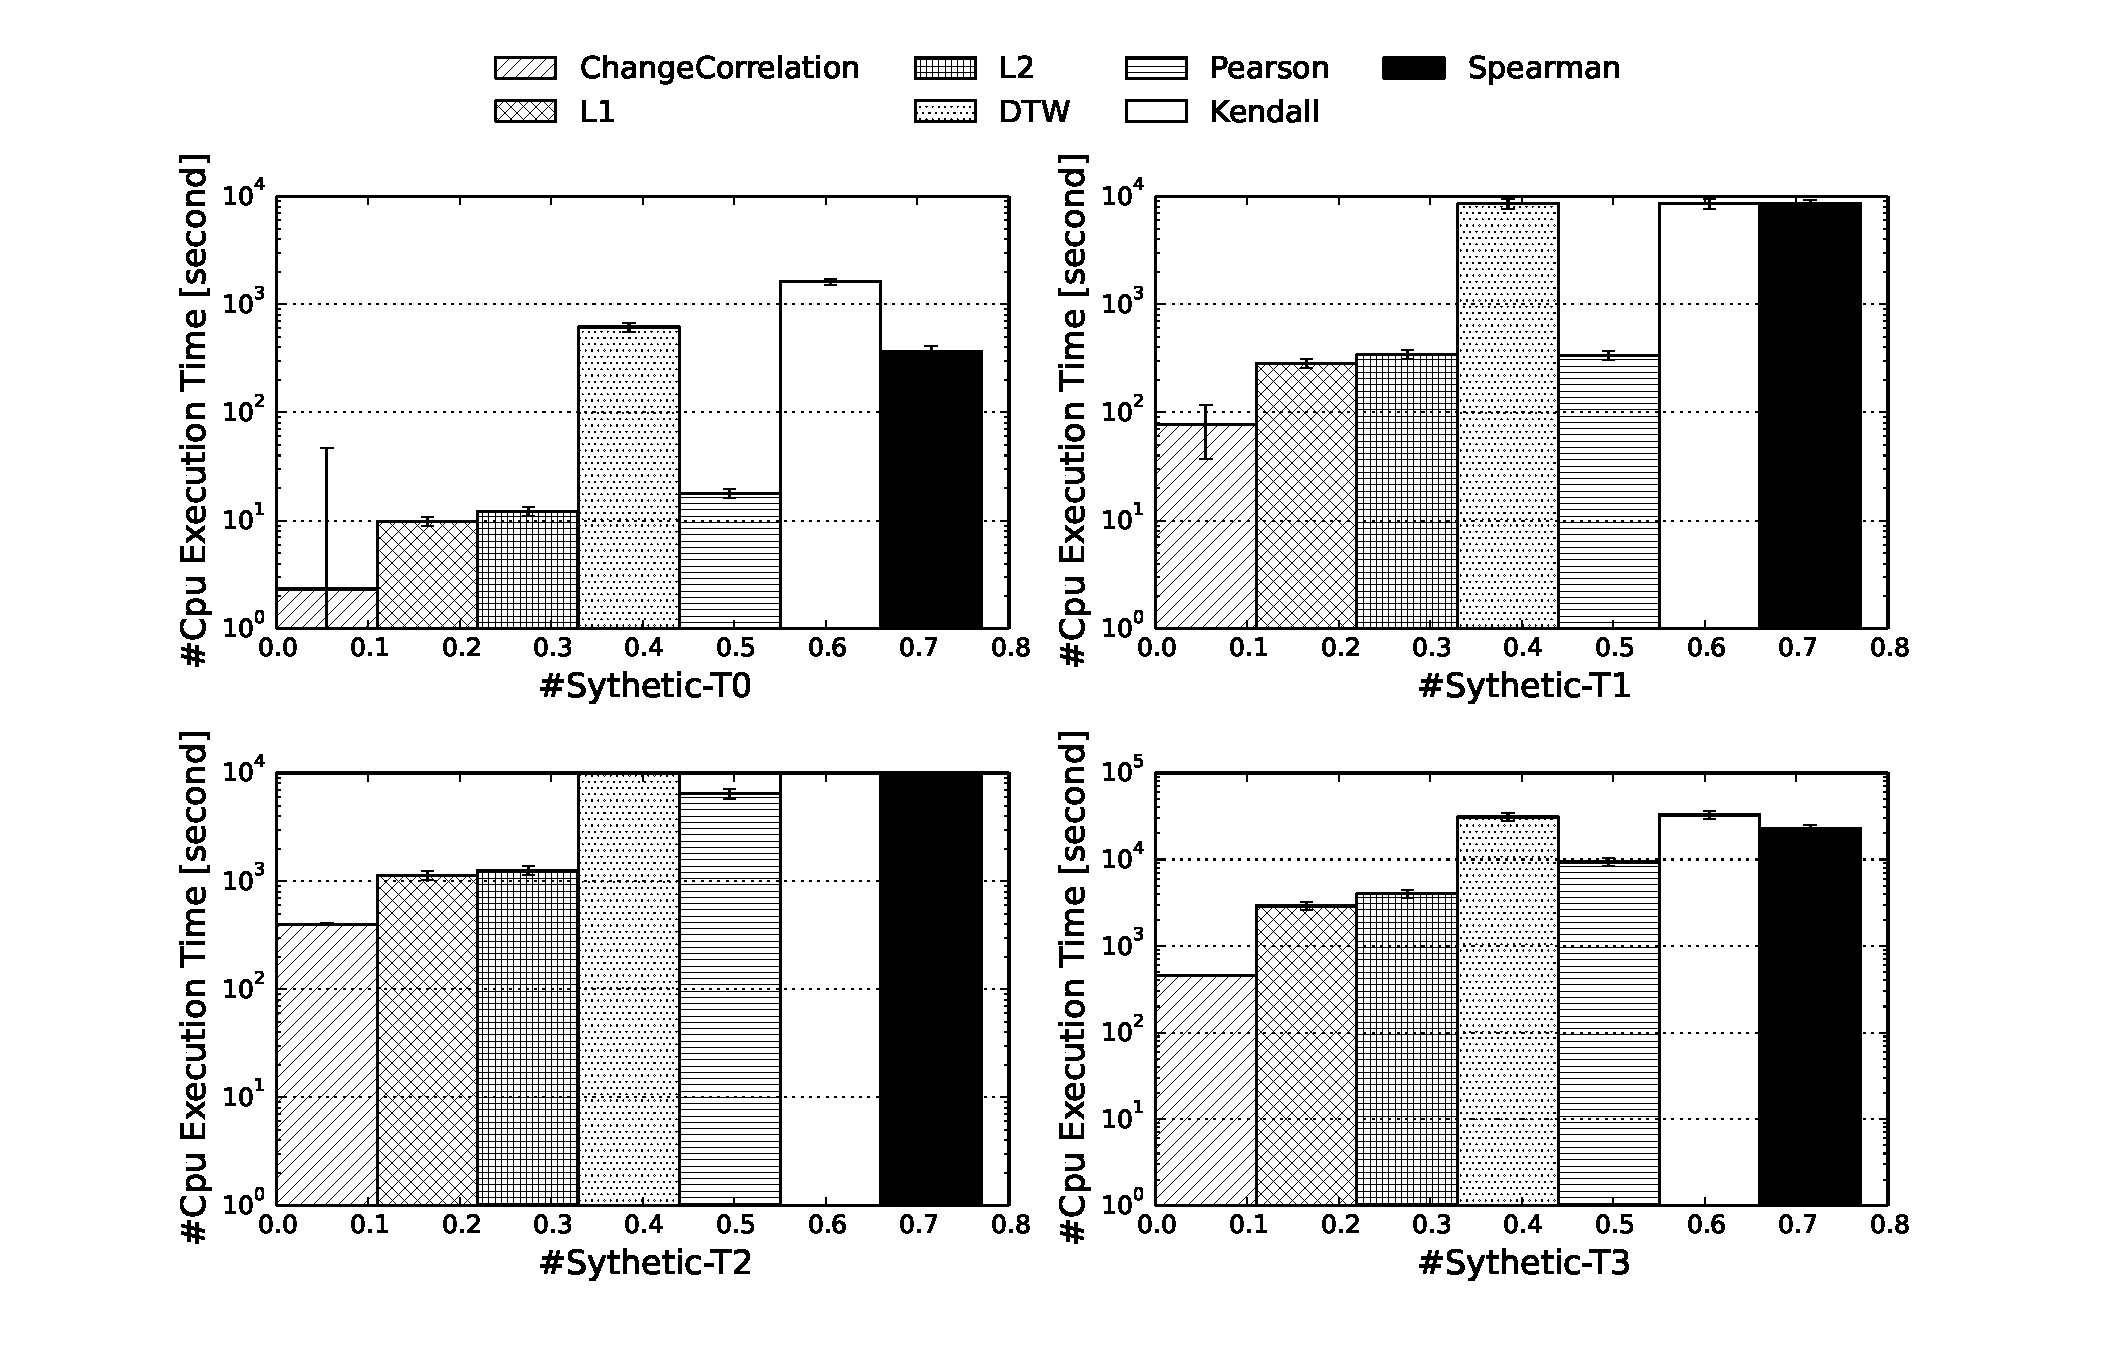
\includegraphics[width=0.8\textwidth]{SythClusPerf.eps}
\caption{Top-k Nearest Neighbor Search}
\label{Fig:ClusPerf}
\end{figure*}

\begin{figure*}[t]
\centering

\subfigure{%
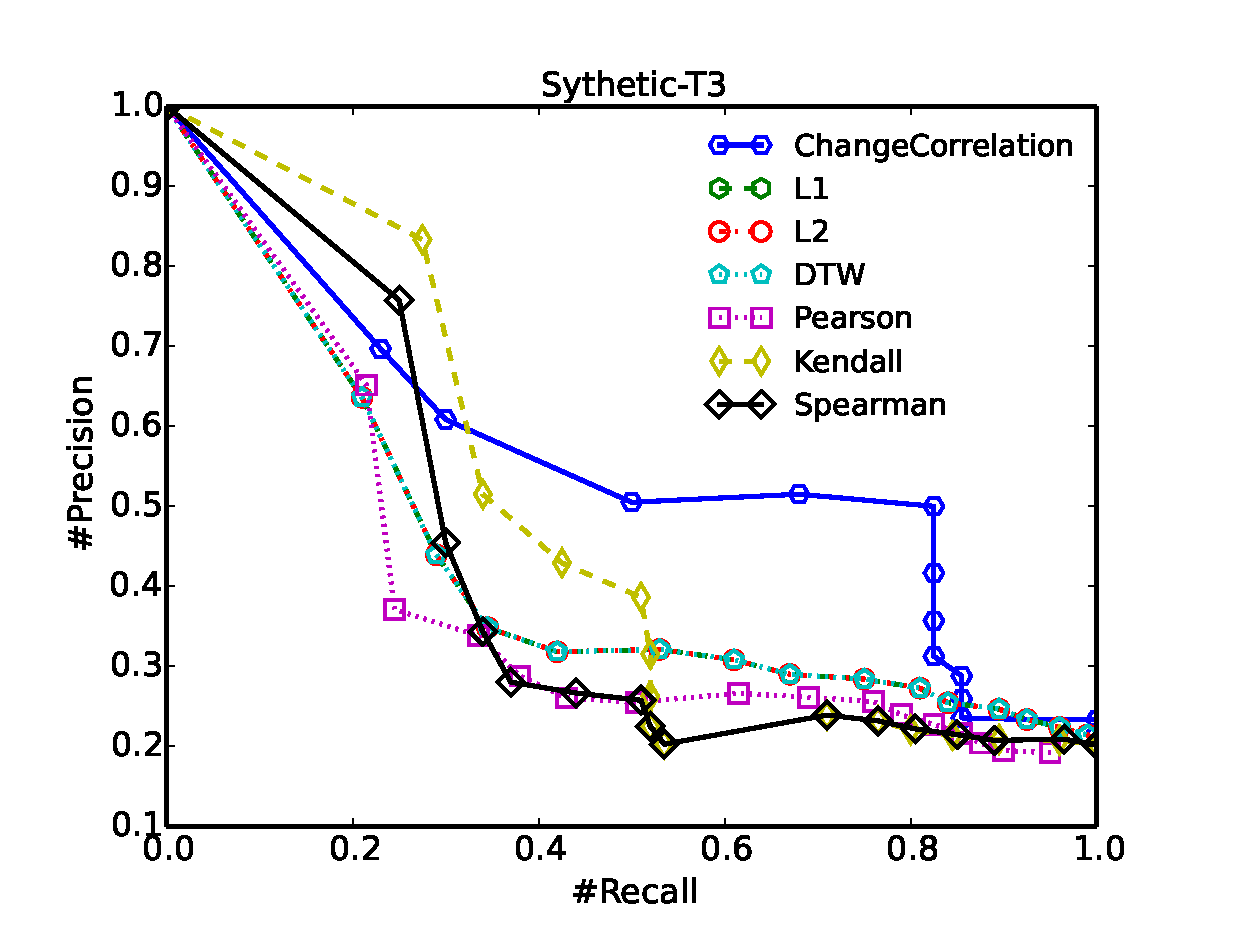
\includegraphics[width=0.41\textwidth]{PRC3.eps}
}\hspace{0.001em}
\subfigure{%
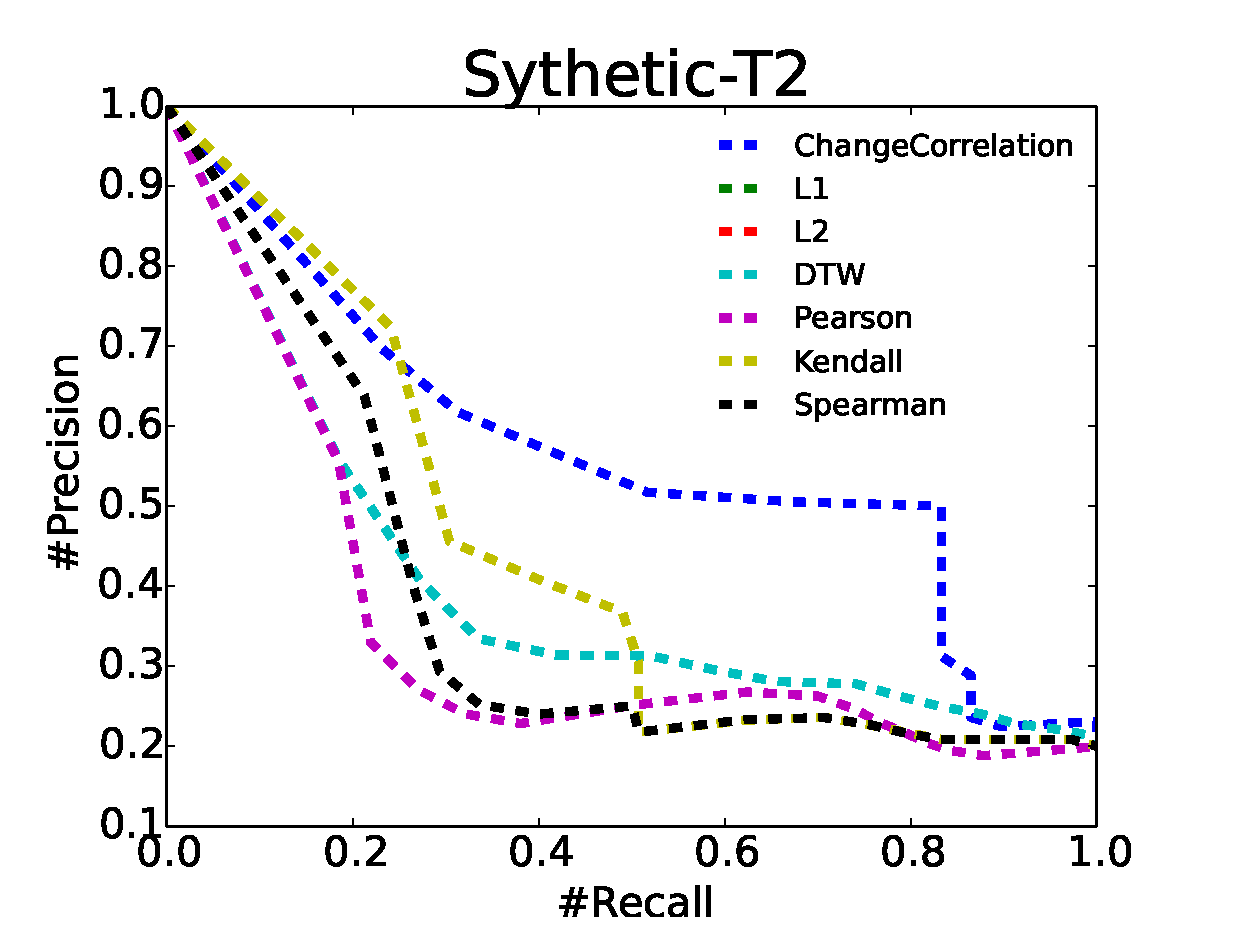
\includegraphics[width=0.41\textwidth]{PRC2.eps}
}\hspace{0.001em}
\subfigure{%
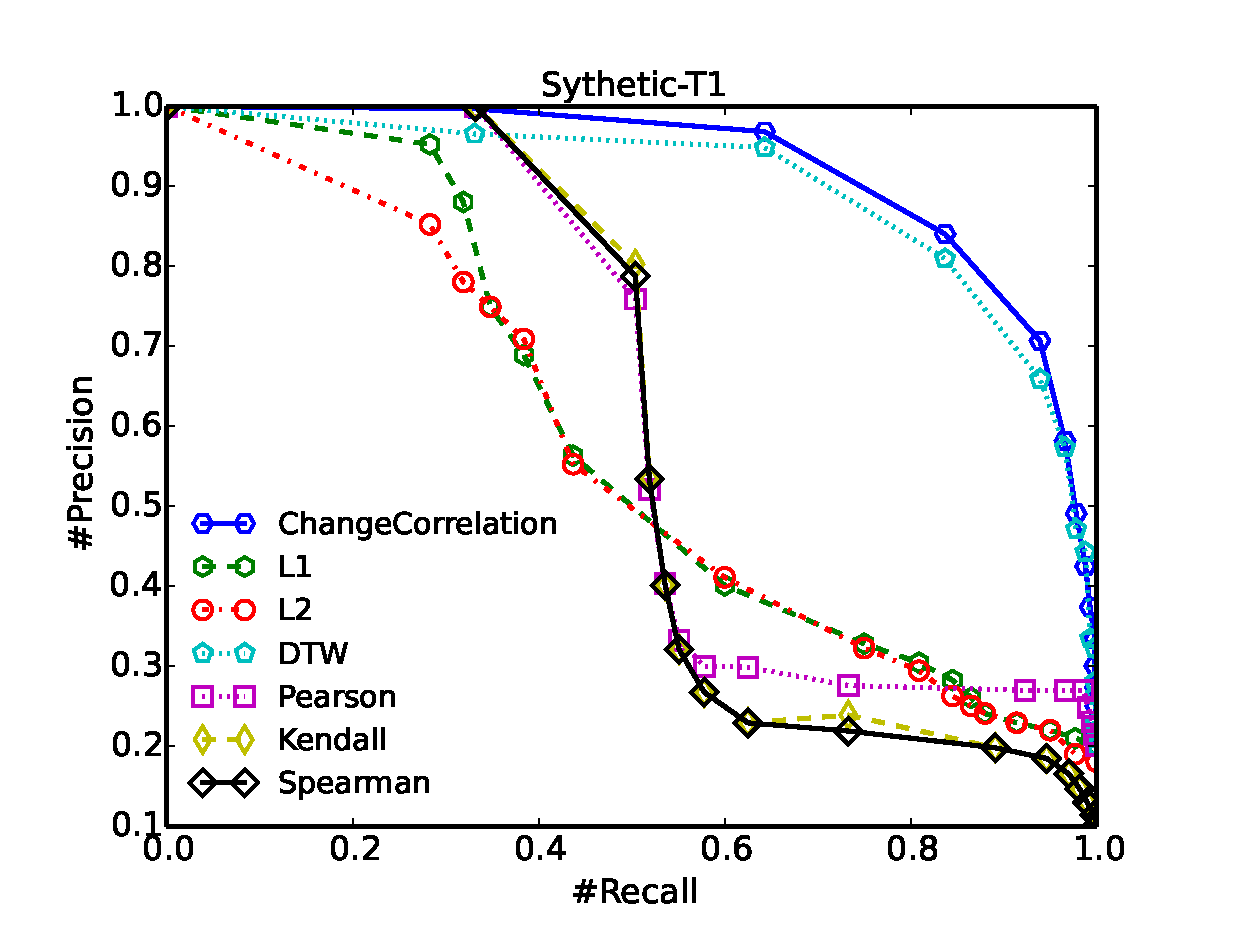
\includegraphics[width=0.41\textwidth]{PRC1.eps}
}\hspace{0.001em}
\subfigure{%
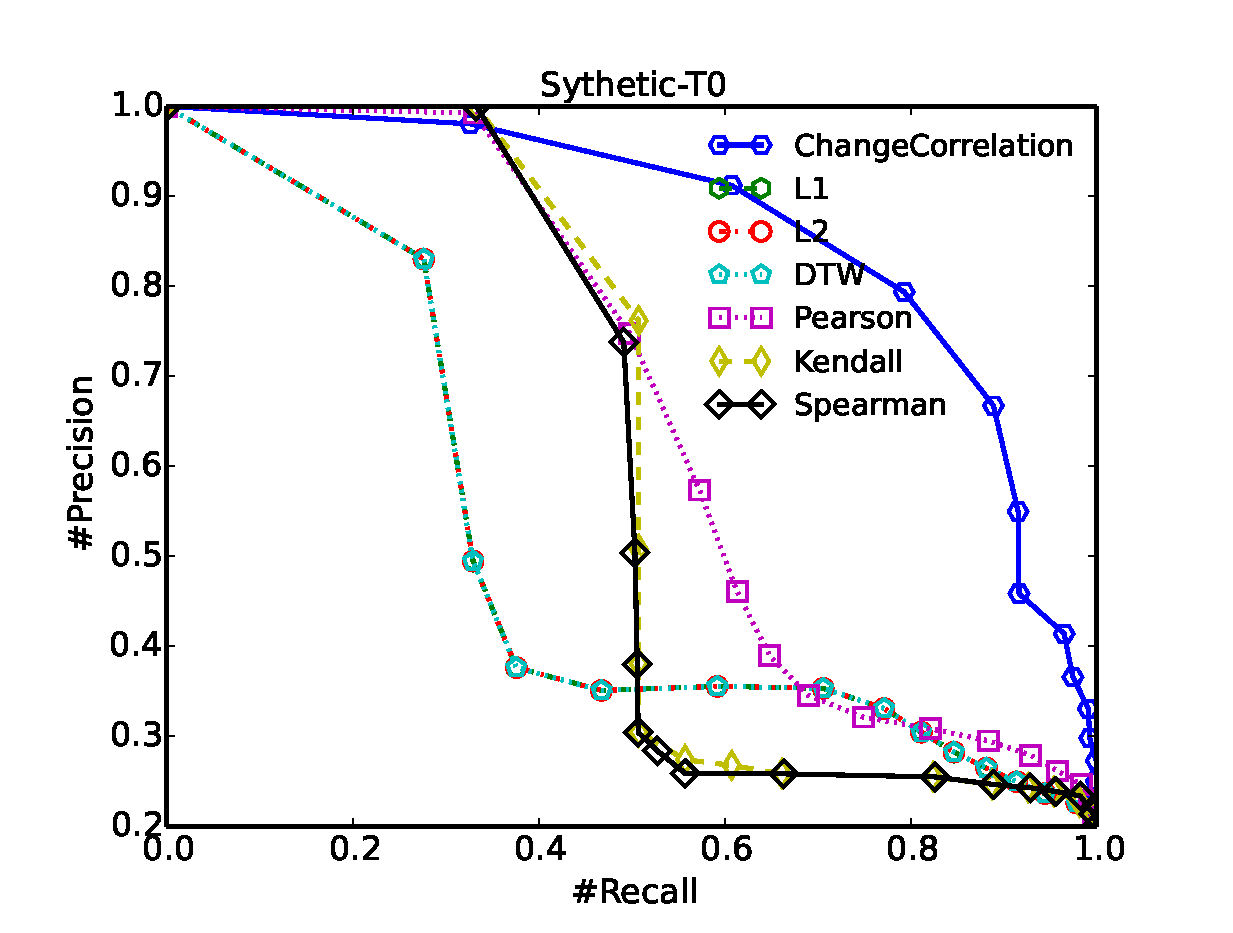
\includegraphics[width=0.41\textwidth]{PRC0.eps}
}
%
\caption{Precision Recall Curve for Different Algorithms}
\label{fig:NNPreRe}
\end{figure*}


\begin{figure*}
\centering
\subfigure{%
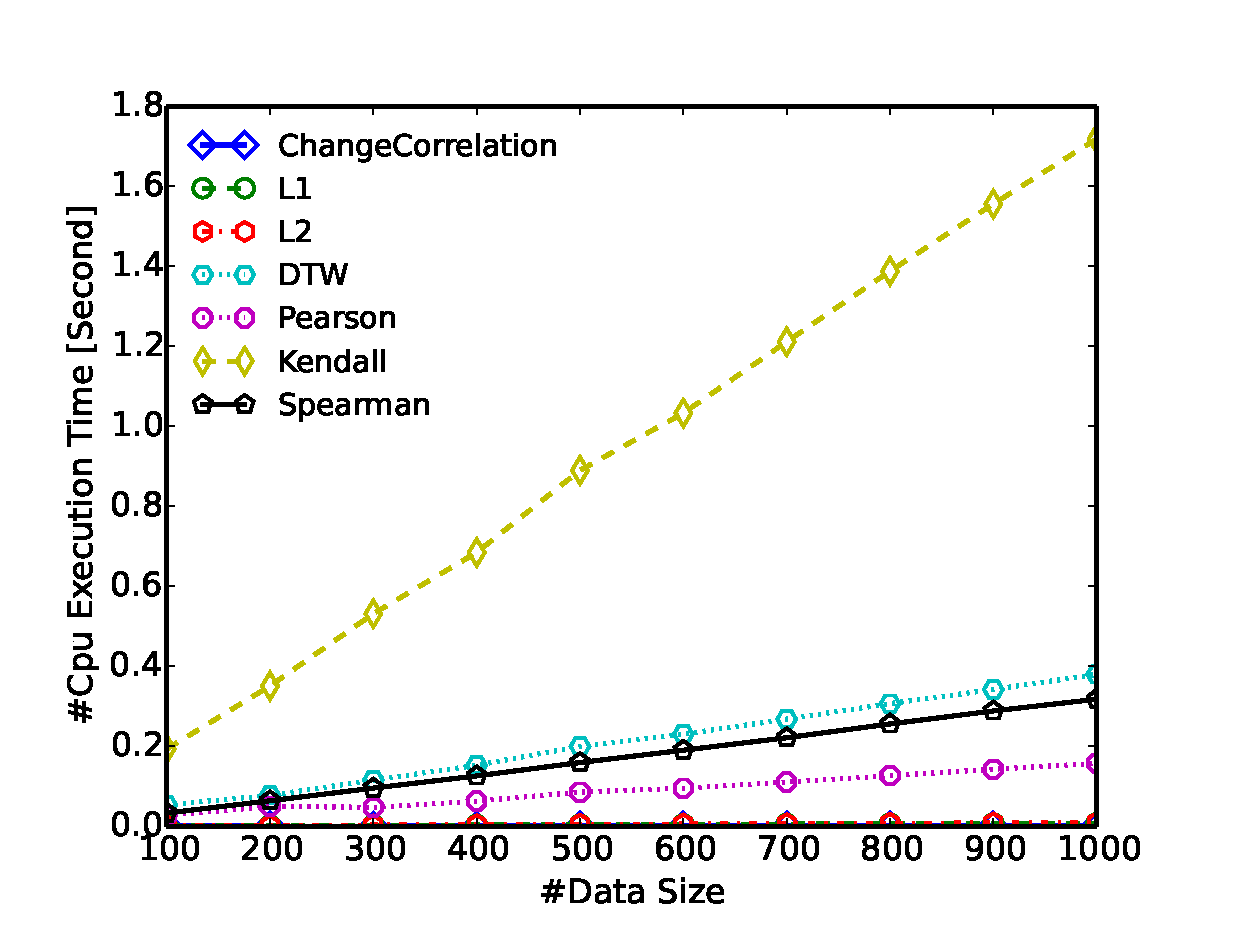
\includegraphics[width=0.45\textwidth]{VaryDataSize.eps}
}\hspace{0.001em}
\subfigure{%
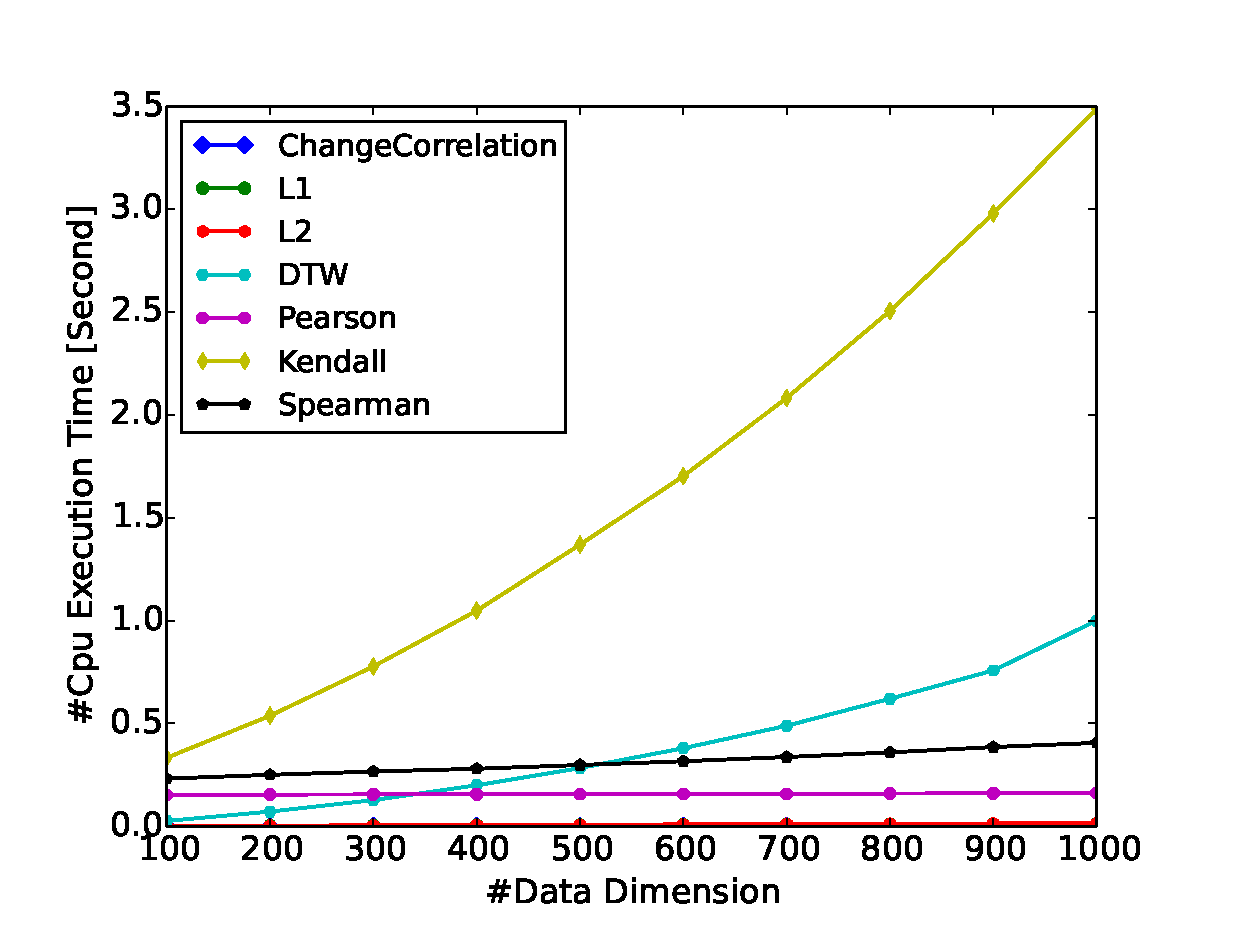
\includegraphics[width=0.45\textwidth]{VaryDataDimension.eps}
}\hspace{0.001em}
\caption{Efficiency by varying data size and dimension size}
\label{fig:NNPerf}
\end{figure*}


\subsubsection{Clustering Task}

In order to evaluate the performance of our correlation coefficient, we design a clustering task. In this experiment, we only use the Hierarchical Clustering \cite{han2011data} to evaluate the clustering performance.

Two evaluation methods are used for testing the clustering result: Accuracy \cite{han2011data}, which is calculated as the percentage of target objects clustered into the correct clusters; and Normalized Mutual Information (NMI) \cite{han2011data}, which is one of the most popular evaluation methods to evaluate the quality of clustering results.

From Table.\ref{Tab:ClusRes}, we can see that, for the change correlation coefficient, the clustering result performance is better for the high dimensional data set.
This is because that for high dimensional time series data, the proposed coefficient can extract more change information from the time series data and also make more accurate evaluation of the correlation. 
From this point of view, change based correlation is more suitable for the high dimensional time series data set.
On the other hand, Change based correlation can obtain more accuracy results in different dataset compared with both the similarity method and the correlation coefficient. So, the result of clustering show the effectiveness of our coefficient.


Fig.\ref{Fig:ClusPerf} shows the Execution time of the clustering task on each data set. From the result, we can see that change based correlation performed much faster than other algorithms. This is because, we only calculate the correlation on the extracted change information (Bit-stream), the calculating of change based correlation measure can be much faster than other similarity and correlation methods.


\subsubsection{K-nearest Neighbors Task}

We compute precision and recall \cite{powers2011evaluation} on the data-set using the LSH method, and other methods using the naive K-nearest Neighbors method. 
If the Searched time series is in the same cluster of the query time series, we regard it as a relevant items, and vice verse. We range the $K$ from $1$ to the cluster size. 

For each top-k Nearest Neighbors search, the precision can be calculated as follow:

\begin{equation}
Precision =\frac{relevant~item}{K} 
\end{equation}

and the recall can be calculated as follow:

\begin{equation}
Precision =\frac{relevant~item}{Relevant~Cluster~Size} 
\end{equation}

The plots for all the three datasets are shown in Figure.\ref{fig:NNPreRe}.
We can clearly see that our proposed Change-based Correlation method gives significantly higher precision recall curves than other similarity and correlation methods. In addition the results are consistent across datasets.

Fig.\ref{fig:NNPerf} shows the execution time by vary the data size and the time series length.
In left one of Fig.\ref{fig:NNPerf}, we fix the value of time series length, and
vary the data size n. We can see that the CPU execution
time of other similarity methods increased sharply by enlarging the data size. 
And, the change based correlation do not change so much by enlarge the data size.

In right of Fig. \ref{fig:NNPerf}, we fix the size of data size, and vary the value of time series length. Based on the results, we can see that the running time of the proposed change based method with LSH doesn't so much with the increase of time series length, while other methods increase by enlarging the time series length.




\subsection{Effectiveness Study on Real Datasets}

In this section, we will compare the proposed algorithm with the baseline algorithms on two real data sets.

\subsubsection{Electrocardiogram Data set}

The first real world dataset is ECG (Electrocardiogram) time series data set. This data set is comming from the the UCR time series Data set Archive \cite{UCRArchive}.

Electrocardiography \cite{holter1961new} (ECG or EKG*) 
is the process of recording the electrical activity of the heart over a period of time using electrodes placed on a patient's body. 
These electrodes detect the tiny electrical changes on the skin that arise from the heart muscle depolarizing during each heartbeat. 
By analyzing such data, one can find some useful information hidden behind the human body, thus to uncover some miracle of human body \cite{tilley1979essentials}.

Such ECG data can be regarded as time series data. Detect the correlation between each ECG time series is a powerful tool to analyze ECG data. After knowing the correlation between different ECG data, we can use such correlation to discover the hidden relation ship between each human and disease \cite{marriott1988practical}.

However, we can see from Fig.\ref{fig:ecgexample} that, ECG time series data correlation are regarded as tiny electrical change at the same time \cite{tilley1979essentials}. And the change has different patterns. As a result, some classical similarity or correlation method can not deal with such problem well, even DTW some times also fail to detect such patterns. As a result, a change based correlation is needed.
\begin{table}
\caption{Summary of the Four ECG Data Set}
\centering

\begin{tabular}{|c|c|c|}
\hline Data Set & \centering Data Size & Time Series Length \\
\hline CinC_ECG_torso & \centering 1380 & 1639 \\
\hline ECGFiveDays & \centering 861 & 136 \\
\hline TwoLeadECG & \centering 1139 & 82 \\
\hline ECG5000 & \centering 4500 & 140 \\
\hline
\end{tabular}
\label{Tab:ECGData}
\end{table}

\begin{table*}[t]
\caption{Clustering Performance on Synthetic ECG Data Set From UCR Time Series Archive}
\centering
\renewcommand{\arraystretch}{1.2}
\begin{tabular}{ccccccccc} 
\toprule[2pt] 
%\hline
Dataset & Measure & Proposed & $L1$ & $L2$ & DTW & Pearson & Kendall & Spearman \\
\toprule[1.5pt] 
\multirow{2}*{\centering{CinC_ECG_torso}}
     & Accuracy & $\boldsymbol{.839\pm.011}$ & $.667\pm.068$ & $.557\pm.012$ & $.610\pm.061$ & $.531\pm.140$ & $.507\pm.019$ & $.504\pm.013$ \\
\cline{2-9}
     & NMI & $\boldsymbol{.489\pm.019}$ & $.236\pm.035$ & $.019\pm.023$ & $.010\pm.075$ & $.280\pm.55$ & $.150\pm.015$ & $.049\pm.012$ \\
\toprule[1.2pt] 
\multirow{2}*{\centering{EGG_5000}}
     & Accuracy & $\boldsymbol{.538\pm.025}$ & $.247\pm.026$ & $.262\pm.032$ & $.283\pm.012$ & $.240\pm.018$ & $.374\pm.067$ & $.341\pm.067$ \\
\cline{2-9}
     & NMI & $\boldsymbol{.401\pm.030}$ & $.003\pm.062$ & $.057\pm.043$ & $.064\pm.036$ & $.046\pm.084$ & $.404\pm.023$ & $.230\pm.042$ \\
\toprule[1.2pt] 
\multirow{2}*{\centering{TwoLeadECG}}
     & Accuracy & $\boldsymbol{.810\pm.029}$ & $.504\pm.066$ & $.538\pm.080$ & $.620\pm.022$ & $.528\pm.064$ & $.531\pm.052$ & $.519\pm.049$ \\
\cline{2-9}
     & NMI & $\boldsymbol{.680\pm.012}$ & $.081\pm.042$ & $.043\pm.056$ & $.137\pm.032$ & $.047\pm.064$ & $.062\pm.052$ & $.074\pm.049$ \\
\toprule[1.2pt] 
\multirow{2}*{\centering{ECGFiveDays}}
     & Accuracy & $\boldsymbol{.832\pm.077}$ & $.502\pm.028$ & $.527\pm.034$ & $.615\pm.062$ & $.506\pm.032$ & $.547\pm.032$ & $.519\pm.032$ \\
\cline{2-9}
     & NMI & $\boldsymbol{.765\pm.017}$ & $.002\pm.040$ & $.002\pm.043$ & $.361\pm.038$ & $.075\pm.032$ & $.023\pm.032$ & $.086\pm.032$ \\
\bottomrule[1.5pt] 
\end{tabular}
\label{Tab:ECGClus}
\end{table*}

\begin{figure*}[t]
\centering
\subfigure{%
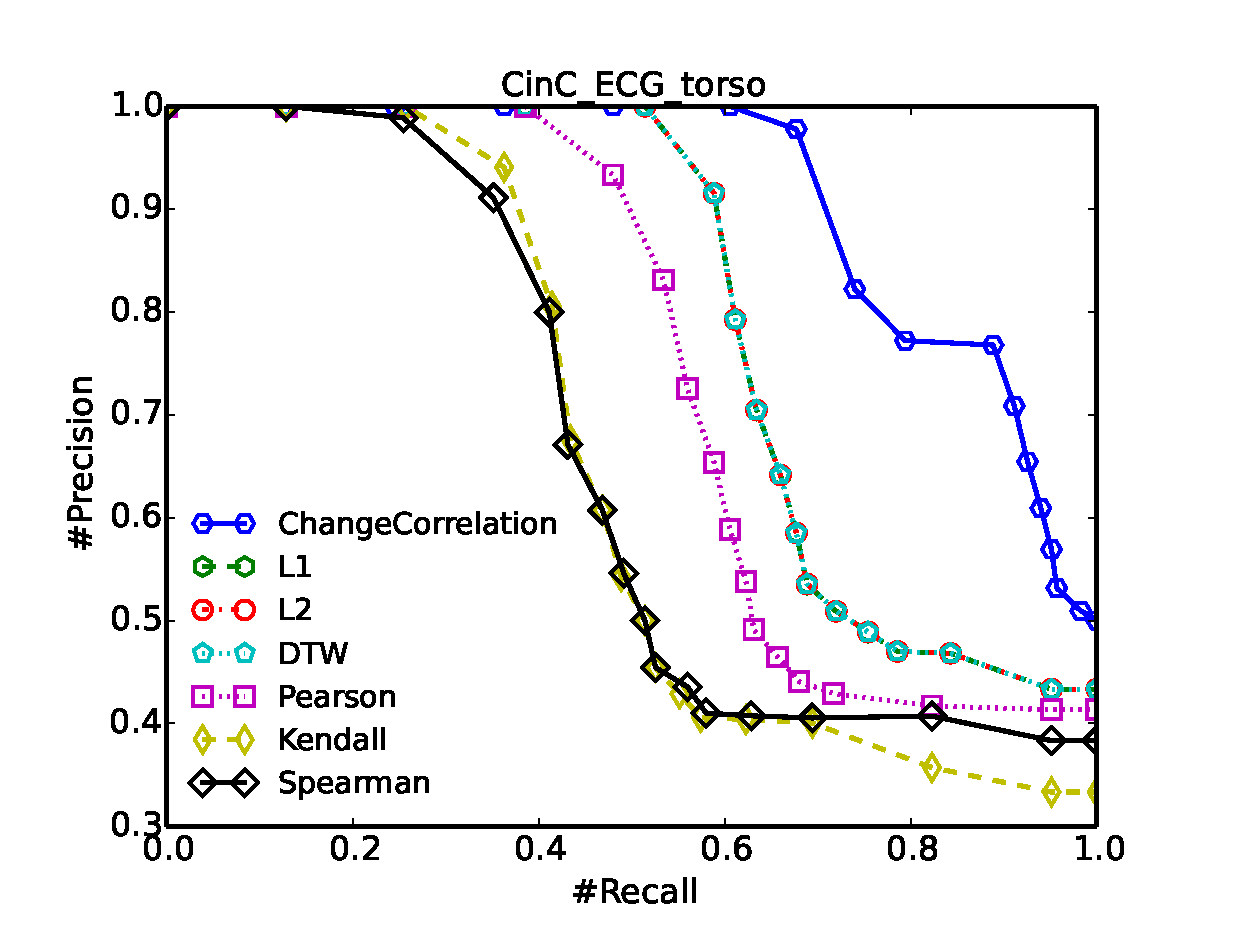
\includegraphics[width=0.45\textwidth]{PRCCinCECGtorso.eps}
}\hspace{0.001em}
\subfigure{%
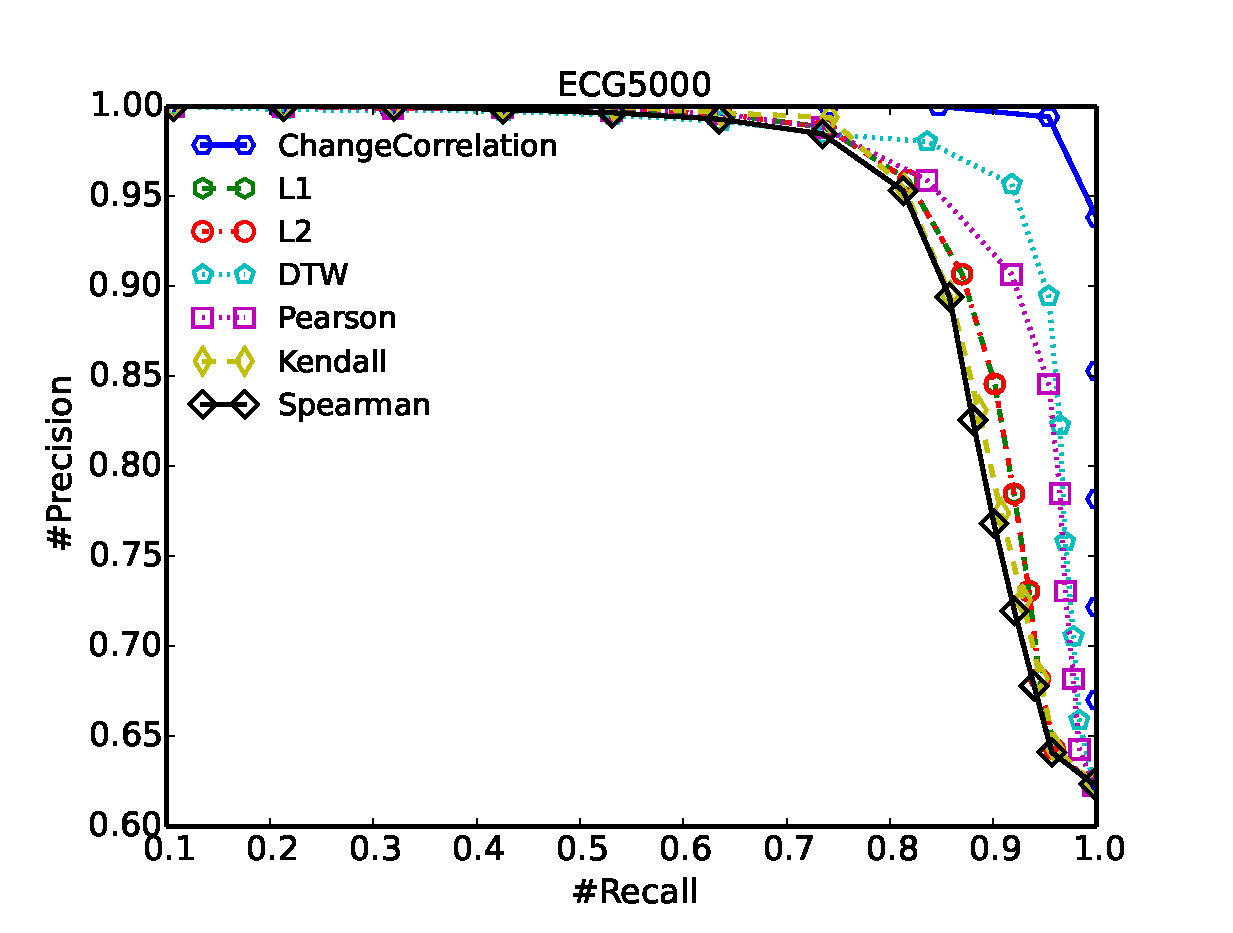
\includegraphics[width=0.45\textwidth]{PRCECG5000.eps}
}\hspace{0.001em}
\subfigure{%
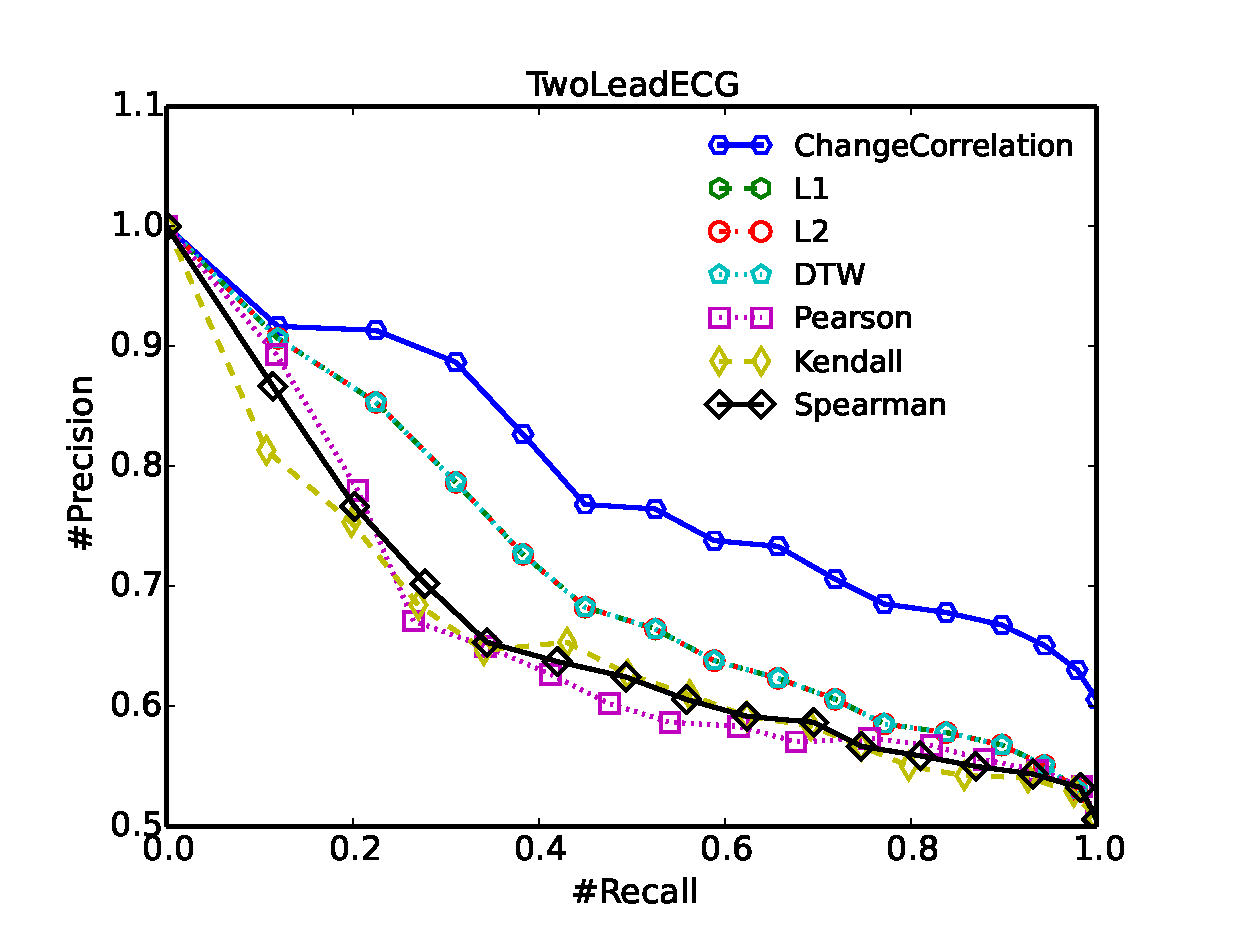
\includegraphics[width=0.45\textwidth]{PRCTwoLeadECG.eps}
}\hspace{0.001em}
\subfigure{%
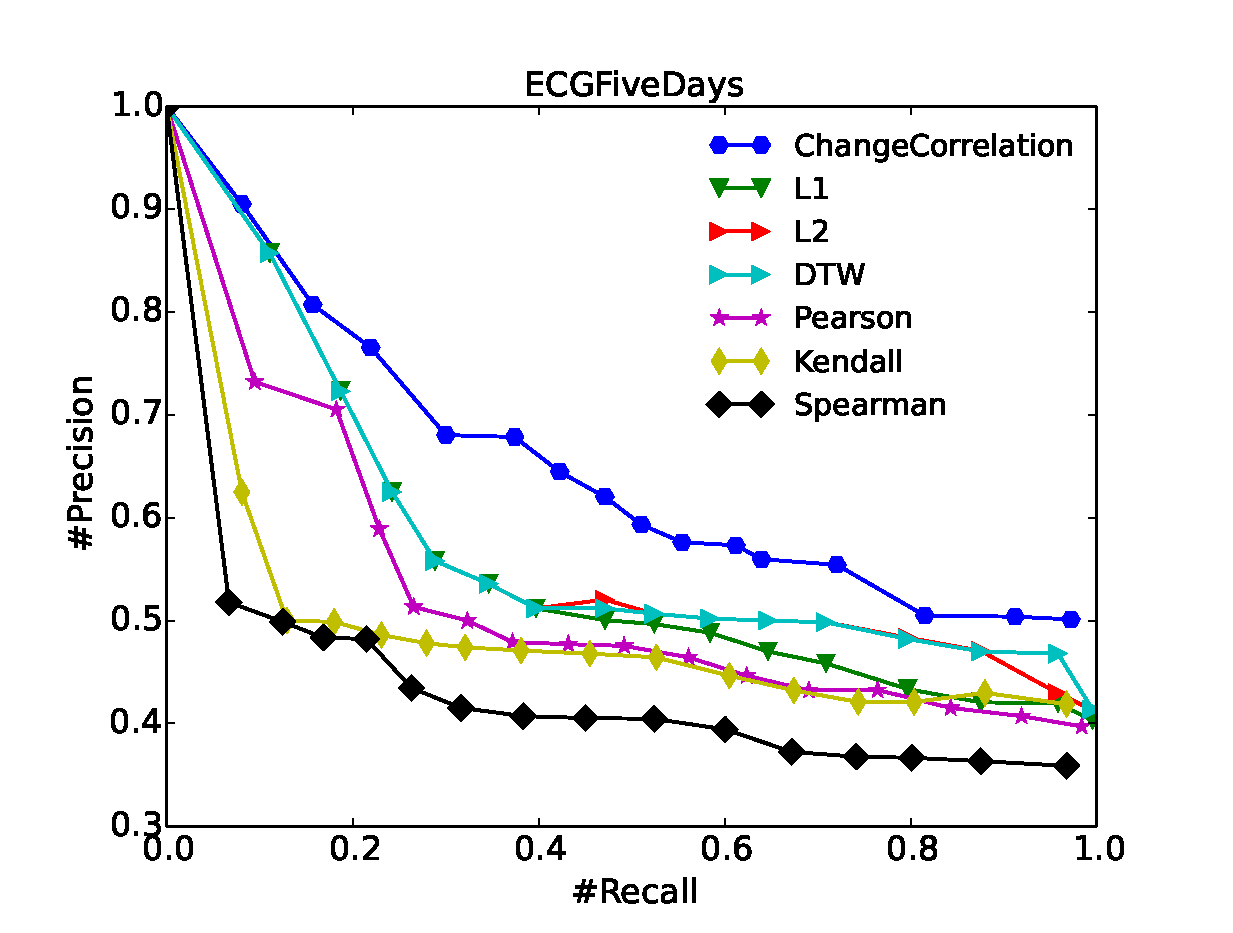
\includegraphics[width=0.45\textwidth]{PRCECGFiveDays.eps}
}\hspace{0.001em}
\caption{Precision Recall Curve (higher is better). We compare Change based correlation coefficient with other methods.}
\label{fig:ECGPRC}
\end{figure*}


\subsubsection{HPC Thread Time Series Data set}

The second real world dataset is from the HPC-tool Kit Dataset.

High performance computers (HPC) have become enormously complex. Today, the largest systems consist of more than tens of thousands of nodes. Nodes themselves are equipped with one or more multicore microprocessors\cite{adhianto2010hpctoolkit}. 

As a result, it is increasingly difficult for application developers writing complex scientific programs to attain a significant fraction of peak performance on modern microprocessor-based computer systems. 
So, how to automatically analysis and monitoring the HPC is a major task for HPC researchers \cite{mccurdy2010memphis,tallent2009effective}.

HPCToolkit\footnote{http://hpctoolkit.org/}, introduced by Dr.John Mellor-Crummey, can generate some performance information of each process (or thread if application is multithreaded.) along the time. So, each process (thread) can be represented as a time series. (Depend on which aspect of a thread to be represent, domain knowledge required) The thread change information (e.g. change from one state to another state) can directly reflect some important properties of different threads. 

Fig. \ref{fig:hpcexample} shows a example of three thread time series data. From the figure, we can see that above two thread often change at same time, so they may have highly correlation with each other. However, using the point to point based similarity method, we can not handle such heterogeneity property of different thread time series.

\begin{table}
\caption{Summary of the HPC Time Series Data Set}
\centering

\begin{tabular}{|c|c|c|}
\hline Data Set & \centering Data Size & Time Series Length \\
\hline Single PC & \centering 24 & 4096 \\
\hline MADNESS & \centering 264 & 32768 \\
\hline
\end{tabular}
\label{Tab:HPCData}
\end{table}

\begin{table*}[t]
\caption{Clustering Performance on Synthetic ECG Data Set From UCR Time Series Archive}
\centering
\renewcommand{\arraystretch}{1.2}
\begin{tabular}{ccccccccc} 
\toprule[2pt] 
%\hline
Dataset & Measure & Proposed & $L1$ & $L2$ & DTW & Pearson & Kendall & Spearman \\
\toprule[1.5pt] 
\multirow{2}*{\centering{Single PC}}
     & Accuracy & $\boldsymbol{.917\pm.011}$ & $.835\pm.068$ & $.815\pm.012$ & $.870\pm.061$ & $.501\pm.140$ & $.527\pm.019$ & $.514\pm.013$ \\
\cline{2-9}
     & NMI & $\boldsymbol{.889\pm.019}$ & $.736\pm.035$ & $.719\pm.023$ & $.860\pm.075$ & $.380\pm.55$ & $.350\pm.015$ & $.349\pm.012$ \\
\toprule[1.2pt] 
\multirow{2}*{\centering{MADNESS}}
     & Accuracy & $\boldsymbol{.938\pm.025}$ & $.927\pm.026$ & $.922\pm.032$ & $.935\pm.012$ & $.457\pm.018$ & $.474\pm.067$ & $.541\pm.067$ \\
\cline{2-9}
     & NMI & $\boldsymbol{.861\pm.030}$ & $.853\pm.062$ & $.857\pm.043$ & $.864\pm.036$ & $.346\pm.084$ & $.404\pm.423$ & $.230\pm.442$ \\
\toprule[1.2pt] 
\end{tabular}
\label{Tab:HPCClus}
\end{table*}

\begin{figure}[t]
\centering
\subfigure{%
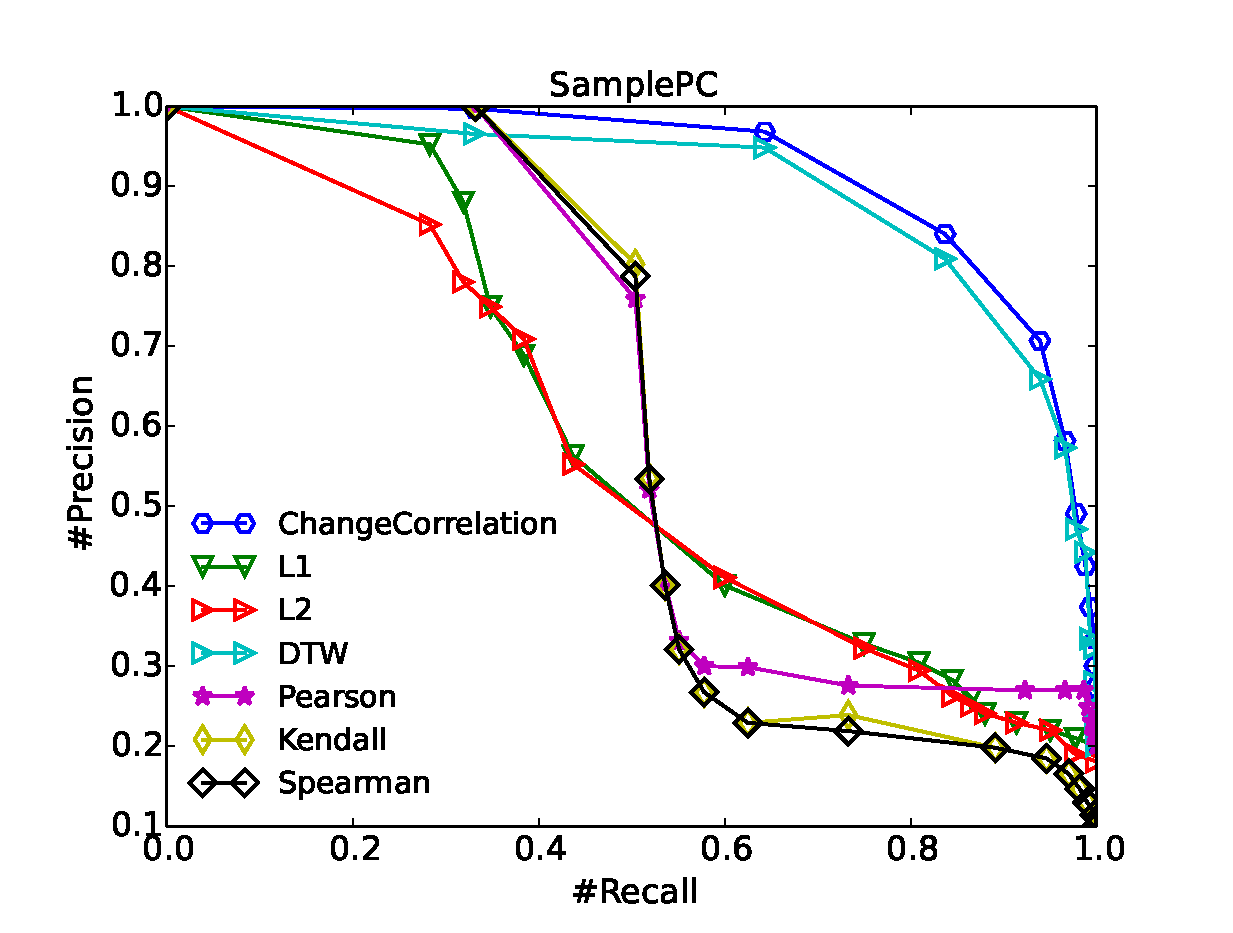
\includegraphics[width=0.45\textwidth]{PRCSamplePC.eps}
}\hspace{0.001em}
\subfigure{%
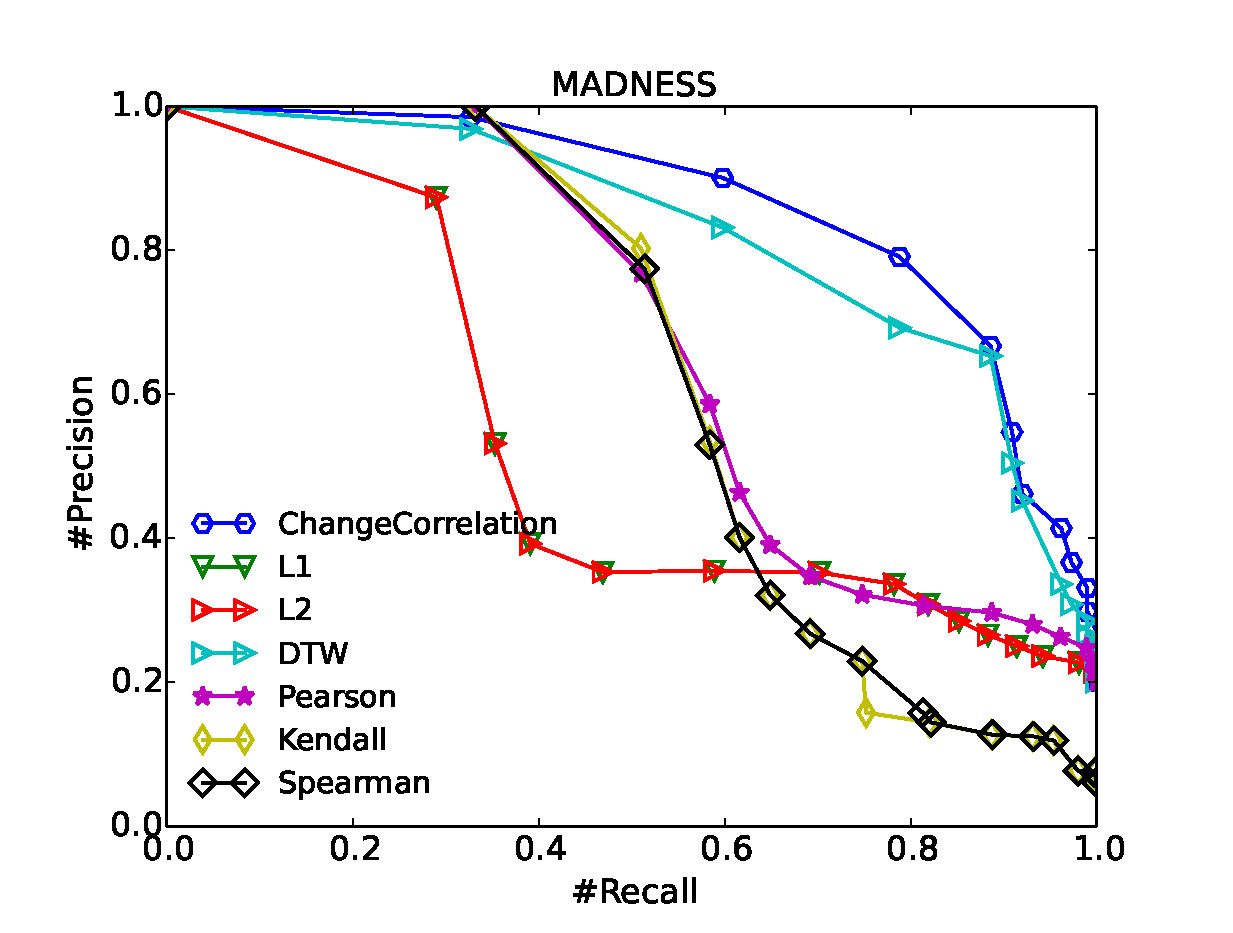
\includegraphics[width=0.45\textwidth]{PRCMADNESS.eps}
}\hspace{0.001em}
\caption{Precision Recall Curve (higher is better). We compare Change based correlation coefficient with other methods.}
\label{fig:HPCPRC}
\end{figure}



